\section{Digit Classification}
\subsection{Part 2.1: Digit Classification with Perceptrons}
\subsubsection{Perceptron Implementation}
\paragraph{Training}
To train the perceptron, we first parse the training examples an array, where each element in the array is a dictionary representing one training example. The dictionary has three key-value pairs: the key ``id'' stores what number example the data belongs to, ``label'' stores the actual label of the object as given in the traininglabels file, and ``image'' stores the digit image as a two-dimensional array. This array of dictionaries is passed to the training algorithm.

We then initialize the weight vectors, of size $28*28=784$, for each of the classes 0-9. Depending on the parameter setting, the weights are either all initialized to zero or to the value of a random variable uniformly distributed between zero and one. Bias is also set, to 0 or 1, depending on the parameter settings entered via command line. Then, for some number of epochs, the training algorithm does the folowing. The learning rate for this epoch is computed; in the default parameter settings, this rate is computed as $\alpha = \frac{1000}{1000+epoch}$. If the parameters were set to randomize the order in which the algorithm reads the training examples, we first shuffle the array of training examples.

Then, the algorithm iterates through the array and computes, for each of the ten classes, $\mathbf{w_c} \cdot \mathbf{x} + b$, where $\mathbf{w_c}$ is the weight vector of class $c$ and $\mathbf{x}$ is the one-dimensional representation of the image. Since the original image contains `` ``, ``+'', and ``\#'', we converted these to numerical values to enable computation of the dot product; the three characters were assigned values 0, 1, and 1, respectively. The algorithm guesses that the training example's label is the class with the highest dot product. If the algorithm guesses correctly, it moves on to the next training example. If not, the algorithm updates, with the following equations, the weight vectors for the example's actual class and the class it was mistaken for:
\begin{equation}
\mathbf{w_c} = \mathbf{w_c} + \alpha{}\mathbf{x}
\end{equation}
updates the weight vector for the example's actual class to increase the dot product when an example from this class has its dot product computed with this class' weight vector. The opposite is done for the weight vector of the class into which this example was mistakenly categorized:
\begin{equation}
\mathbf{w_c} = \mathbf{w_c} - \alpha{}\mathbf{x}
\end{equation}

This is done for all of the training examples in the training examples array. The algorithm then moves on to the next epoch, recalculates the learning rate $\alpha$, and repeates the above steps for the training examples.

\paragraph{Testing}
The weight vectors are then passed to the testing algorithm. The algorithm iterates the test examples, and for each example, the algorithm computes the dot product $\mathbf{w_c} \cdot \mathbf{x}$, where $\mathbf{w_c}$ is the weight vector for class $c$ and $\mathbf{x}$ is the one-dimensional representation of the test example image, for each of the ten classes. Its label estimate for a given test example is the class with the largest dot product. The testing algorithm repeats this process for all of the testing examples.


\subsubsection{Parameter Settings}
We first tried our default settings, where we initialized the weights to zero, fix the order of the training examples, did not use bias, and trained for ten epochs; the learning rate decay function we used was $\alpha = \frac{1000}{10
00+epoch}$. We noted that the accuracy on the training set stabilized after the second epoch, so we decided not to try increasing the number of epochs used. Additionally, these default settings yielded an accuracy greater than 75\% (82.3\%), so we tried very few other settings, as detailed below.

Then, we randomized the order of the training examples without changing the other parameters and found that this decreased the accuracy. Therefore, we reverted to fixing the training examples order and instead initialized the weights to random values. This dec the accuracy, compared to the accuracy yielded by our default settings, so we revert to initializing our weights to zero.

As stated above, we chose not to increase the number of epochs used, so we finally varied the learning rate decay function. Over ten epochs, with weights initialized to zero and the order of training examples fixed, we substituted $\alpha = \frac{100}{100+epoch}$ for our decay function. The accuracy remained 82.3\%.

Since our default settings yielded the best results, we will show below the data generated from those parameters.

\subsubsection{Training Curve}
\begin{tabular}{l|r}
Epoch number & Accuracy on training set \\
\hline
1 & 0.7814 \\
2 & 0.8602 \\
3 & 0.8602 \\
4 & 0.8602 \\
5 & 0.8602 \\
6 & 0.8602 \\
7 & 0.8602 \\
8 & 0.8602 \\
9 & 0.8602 \\
10 & 0.8602 \\
\end{tabular}

\subsubsection{Overall Accuracy}
The overall accuracy of the perceptron on the test set was 79\%.

\subsubsection{Confusion Matrix}
\paragraph{Left side of matrix}

\begin{tabular}{l|r|r|r|r|r}
 & 0 & 1 & 2 & 3 & 4 \\
\hline
0 & 0.8444444444 & 0.0000000000 & 0.0888888889 & 0.0000000000 & 0.0000000000 \\
1 & 0.0000000000 & 0.9351851852 & 0.0185185185 & 0.0000000000 & 0.0092592593 \\
2 & 0.0000000000 & 0.0097087379 & 0.9320388350 & 0.0000000000 & 0.0097087379 \\
3 & 0.0000000000 & 0.0000000000 & 0.1200000000 & 0.6300000000 & 0.0000000000 \\
4 & 0.0000000000 & 0.0000000000 & 0.0654205607 & 0.0000000000 & 0.7476635514 \\
5 & 0.0108695652 & 0.0000000000 & 0.0217391304 & 0.0217391304 & 0.0000000000 \\
6 & 0.0109890110 & 0.0109890110 & 0.0769230769 & 0.0000000000 & 0.0219780220 \\
7 & 0.0000000000 & 0.0377358491 & 0.1132075472 & 0.0000000000 & 0.0094339623 \\
8 & 0.0097087379 & 0.0291262136 & 0.1456310680 & 0.0194174757 & 0.0291262136 \\
9 & 0.0000000000 & 0.0000000000 & 0.0300000000 & 0.0000000000 & 0.0200000000 \\
\end{tabular}

\paragraph{Right side of matrix}

\begin{tabular}{l|r|r|r|r|r}
0 & 0.0333333333 & 0.0222222222 & 0.0000000000 & 0.0000000000 & 0.0111111111 \\
1 & 0.0000000000 & 0.0092592593 & 0.0000000000 & 0.0277777778 & 0.0000000000 \\
2 & 0.0000000000 & 0.0194174757 & 0.0000000000 & 0.0000000000 & 0.0291262136 \\
3 & 0.1600000000 & 0.0200000000 & 0.0300000000 & 0.0000000000 & 0.0400000000 \\
4 & 0.0000000000 & 0.0373831776 & 0.0000000000 & 0.0373831776 & 0.1121495327 \\
5 & 0.8478260870 & 0.0543478261 & 0.0108695652 & 0.0326086957 & 0.0000000000 \\
6 & 0.0219780220 & 0.8461538462 & 0.0109890110 & 0.0000000000 & 0.0000000000 \\
7 & 0.0094339623 & 0.0000000000 & 0.6226415094 & 0.0188679245 & 0.1886792453 \\
8 & 0.0970873786 & 0.0388349515 & 0.0097087379 & 0.6116504854 & 0.0097087379 \\
9 & 0.0500000000 & 0.0000000000 & 0.0000000000 & 0.0000000000 & 0.9000000000 \\
\end{tabular}

\subsubsection{Accuracy Comparison with Naive Bayes}
Compared with the Naive Bayes method, perceptron method yields higher overall test set accuracies (up to 79\% for the parameter settings we tried) than Naive Bayes (77.1\%).


\subsection{Part 2.2: Digit Classification with Nearest Neighbor}
\subsubsection{Distance/similarity function}
We return for the distance between two 2D-array representations of images the sum of the distances between each pair of pixels (i,j) from the two images. For two same-sized images, we iterate through each pixel (i,j) and compare the character at (i,j) for the two images.

The characters can be the white pixel ' ', the gray pixel '+', or the black pixel '\#'. If the (i,j) pixels for the two images are one intensity apart, i.e. a white and a gray pixel or a gray and a black pixel, then the distance between the two pixels is one. If they are two intensities apart, i.e. a white and a black pixel, the distance is two. Otherwise, the distance is 0.

The distance between each pair of pixels (i,j) for the two images is summed across all pixels, and the resulting sum is returned as the distance between the two images.

\subsubsection{Overall test set accuracy as a function of k}
Our overall test set accuracy appears to increase with increasing values of $k$ until $k=4$, where the accuracy levels off, begins decreasing, and then fluctuates minimally. Since each run of nearest-neighbors takes about ten minutes, we limited the range of $k$ values to between 1 and 10, inclusive. Below, we show the overall accuracies obtained by our nearest-neighbors algorithm for the $k$ values tried.

\begin{tabular}{l|r}
k & overall accuracy \\
\hline
1 & 0.103 \\
2 & 0.459 \\
3 & 0.870 \\
4 & 0.896 \\
5 & 0.883 \\
6 & 0.888 \\
7 & 0.883 \\
8 & 0.879 \\
9 & 0.880 \\
10 & 0.881 \\
\end{tabular}


\subsubsection{Confusion matrix}
For $k \in \{1,...,10\}$, the $k$ that yielded the best accuracy was $k=4$. The confusion matrix for this $k$ is
\paragraph{Left half of matrix\\}
\begin{tabular}{l|r|r|r|r|r}
actual class \ class confused for & 0 & 1 & 2 & 3 & 4 \\
\hline
0 & 1.0000000000 & 0.0000000000 & 0.0000000000 & 0.0000000000 & 0.0000000000 \\
1 & 0.0000000000 & 1.0000000000 & 0.0000000000 & 0.0000000000 & 0.0000000000 \\
2 & 0.0097087379 & 0.0388349515 & 0.9417475728 & 0.0000000000 & 0.0000000000 \\
3 & 0.0000000000 & 0.0100000000 & 0.0300000000 & 0.8400000000 & 0.0000000000 \\
4 & 0.0000000000 & 0.0186915888 & 0.0000000000 & 0.0000000000 & 0.9252336449 \\
5 & 0.0108695652 & 0.0000000000 & 0.0000000000 & 0.0652173913 & 0.0000000000 \\
6 & 0.0000000000 & 0.0109890110 & 0.0000000000 & 0.0000000000 & 0.0109890110 \\
7 & 0.0094339623 & 0.0943396226 & 0.0094339623 & 0.0000000000 & 0.0094339623 \\
8 & 0.0291262136 & 0.0097087379 & 0.0776699029 & 0.0097087379 & 0.0291262136 \\
9 & 0.0100000000 & 0.0100000000 & 0.0100000000 & 0.0200000000 & 0.0300000000 \\
\end{tabular}

\paragraph{Right half of matrix\\}
\begin{tabular}{l|r|r|r|r|r}
actual class \ class confused for & 5 & 6 & 7 & 8 & 9 \\
\hline
0 & 0.0000000000 & 0.0000000000 & 0.0000000000 & 0.0000000000 & 0.0000000000 \\
1 & 0.0000000000 & 0.0000000000 & 0.0000000000 & 0.0000000000 & 0.0000000000 \\
2 & 0.0000000000 & 0.0000000000 & 0.0097087379 & 0.0000000000 & 0.0000000000 \\
3 & 0.0500000000 & 0.0000000000 & 0.0200000000 & 0.0400000000 & 0.0100000000 \\
4 & 0.0000000000 & 0.0093457944 & 0.0093457944 & 0.0000000000 & 0.0373831776 \\
5 & 0.8369565217 & 0.0434782609 & 0.0108695652 & 0.0108695652 & 0.0217391304 \\
6 & 0.0109890110 & 0.9670329670 & 0.0000000000 & 0.0000000000 & 0.0000000000 \\
7 & 0.0000000000 & 0.0000000000 & 0.8396226415 & 0.0000000000 & 0.0377358491 \\
8 & 0.0388349515 & 0.0097087379 & 0.0194174757 & 0.7378640777 & 0.0388349515 \\
9 & 0.0100000000 & 0.0000000000 & 0.0200000000 & 0.0100000000 & 0.8800000000 \\
\end{tabular}


\subsubsection{Running time}
As mentioned above, each run of nearest-neighbors took approximately ten minutes. From the runtimes, shown below, it appears that runtime is independent of $k$; the time spent on each run was approximately the same for each $k$ we tried. Testing took up almost all of the running time, with training taking less than half a second.

\begin{tabular}{l|r|r}
k & training time (s) & testing time (s) \\
\hline
1 & 0.276668071747 & 600.793694019 \\
2 & 0.273632049561 & 591.041094065 \\
3 & 0.281835794449 & 603.412753105 \\
4 & 0.284846067429 & 640.848700047 \\
5 & 0.272377967834 & 607.270968914 \\
6 & 0.277801036835 & 594.610415936 \\
7 & 0.272485971451 & 595.855957985 \\
8 & 0.269151210785 & 599.931087971 \\
9 & 0.270743846893 & 593.337001801 \\
10 & 0.268632888794 & 597.763916969 \\
\end{tabular}


\subsubsection{Accuracy comparison}
\paragraph{Naive Bayes} Compared with the Naive Bayes method, nearest-neighbors yields higher overall test set accuracies (up to 89.6\%) than Naive Bayes (77.1\%) when the former uses at least three neighbors to estimate test example labels.

\paragraph{Perceptron} Compared with the perceptron method, nearest-neighbors also yields higher overall test set accuracies than the perceptron (up to 79\%) when the former uses at least three neighbors to estimate test example labels.


\subsection{Extra Credit}
For bonus points, we have experimented with ternary-value features. We have also visualized the perceptron weight vectors for each class.

\subsubsection{Ternary-value variables with perceptron} Instead of converting the three types of characters in the images to values of 0, 1, and 1 for `` ``, ``+'', and ``\#'', we convert them to 0, 1, and 2, respectively. This improved the overall test set accuracy to 82.3\%. The training curve and confusion matrix are shown below.
\paragraph{Training Curve\\}
\begin{tabular}{l|r}
Epoch number & Accuracy on training set \\
\hline
1 & 0.792 \\
2 & 0.8868 \\
3 & 0.8868 \\
4 & 0.8868 \\
5 & 0.8868 \\
6 & 0.8868 \\
7 & 0.8868 \\
8 & 0.8868 \\
9 & 0.8868 \\
10 & 0.8868 \\
\end{tabular}

\paragraph{Confusion Matrix}
\paragraph{Left side of matrix}

\begin{tabular}{l|r|r|r|r|r}
 & 0 & 1 & 2 & 3 & 4 \\
\hline
0 & 0.9333333333 & 0.0000000000 & 0.0111111111 & 0.0000000000 & 0.0000000000 \\
1 & 0.0000000000 & 0.9722222222 & 0.0000000000 & 0.0000000000 & 0.0092592593 \\
2 & 0.0000000000 & 0.0194174757 & 0.8446601942 & 0.0000000000 & 0.0097087379 \\
3 & 0.0100000000 & 0.0000000000 & 0.0800000000 & 0.6300000000 & 0.0000000000 \\
4 & 0.0093457944 & 0.0093457944 & 0.0280373832 & 0.0000000000 & 0.8691588785 \\
5 & 0.0434782609 & 0.0000000000 & 0.0000000000 & 0.0108695652 & 0.0108695652 \\
6 & 0.0329670330 & 0.0109890110 & 0.0879120879 & 0.0000000000 & 0.0329670330 \\
7 & 0.0094339623 & 0.0566037736 & 0.0754716981 & 0.0000000000 & 0.0094339623 \\
8 & 0.0194174757 & 0.0291262136 & 0.0388349515 & 0.0097087379 & 0.0097087379 \\
9 & 0.0100000000 & 0.0000000000 & 0.0000000000 & 0.0100000000 & 0.0400000000 \\
\end{tabular}

\paragraph{Right side of matrix}

\begin{tabular}{l|r|r|r|r|r}
 & 5 & 6 & 7 & 8 & 9 \\
\hline
0 & 0.0000000000 & 0.0111111111 & 0.0000000000 & 0.0444444444 & 0.0000000000 \\
1 & 0.0000000000 & 0.0092592593 & 0.0000000000 & 0.0092592593 & 0.0000000000 \\
2 & 0.0000000000 & 0.0388349515 & 0.0388349515 & 0.0485436893 & 0.0000000000 \\
3 & 0.1100000000 & 0.0100000000 & 0.0800000000 & 0.0800000000 & 0.0000000000 \\
4 & 0.0000000000 & 0.0373831776 & 0.0000000000 & 0.0186915888 & 0.0280373832 \\
5 & 0.8152173913 & 0.0217391304 & 0.0108695652 & 0.0869565217 & 0.0000000000 \\
6 & 0.0000000000 & 0.8241758242 & 0.0109890110 & 0.0000000000 & 0.0000000000 \\
7 & 0.0000000000 & 0.0000000000 & 0.7735849057 & 0.0094339623 & 0.0660377358 \\
8 & 0.0679611650 & 0.0291262136 & 0.0194174757 & 0.7766990291 & 0.0000000000 \\
9 & 0.0300000000 & 0.0000000000 & 0.0600000000 & 0.0600000000 & 0.7900000000 
\end{tabular}

\subsubsection{Perceptron weight visualization}
Below is the colormap visualization of the weight vectors for each class, where the classes are along the vertical axis and the feature numbers are along horizontal one.

\paragraph{Discriminative locations/features} Weights that are near zero are less important than those with larger absolute values since the former would add less to the dot product $\mathbf{w_c} \cdot \mathbf{x}$. The less important features, as determined by the colormap, are the first and last few rows of the images, where most of the images merely have blank characters and appear as pale green. More important features appear in the middle region where yellows and pale blues appear in the colormap. The most important features with the largest absolute values of weights appear in a region of dark blues or reds near the middle, though the exact location varies between classes. For example, the colormap shows a region with deep blue in the features ranging from 400 to 500 for class 0, while a similar blue region appears in the features ranging from 300 to 400 for class 2.

\paragraph{Signs of the weights} For some class $c$, negative weights (in cold colors) at a feature (i,j) suggest that having a '+' or '\#' there, represented with value 1 in our perceptron implementation, causes the algorithm to move away from classifying the example as class $c$ since it reduces the dot product $\mathbf{w_c} \cdot \mathbf{x}$. Positive weights, since the values in $\mathbf{x}$ are always non-negative, increase the value of the dot product and make it more likely that the algorithm will classify the example as class $c$.

\begin{figure}[H]
\centering
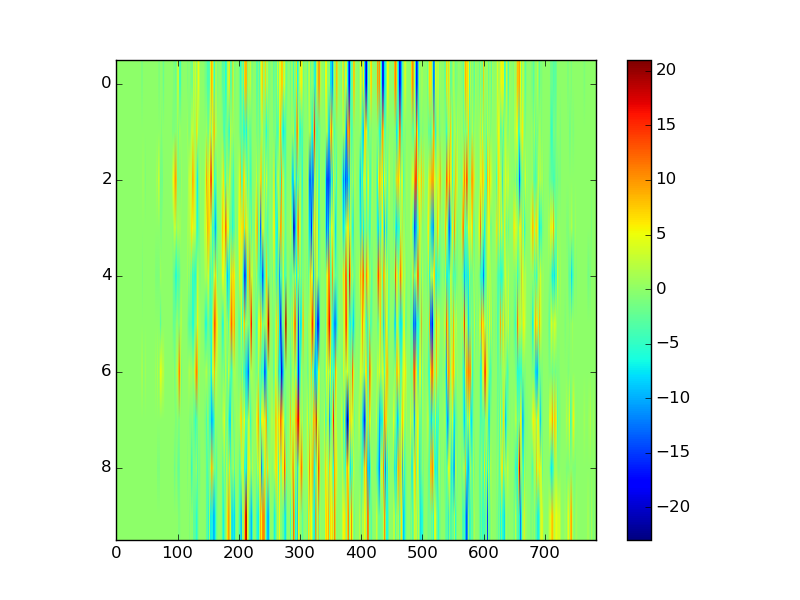
\includegraphics[width=1\textwidth]{graphics/weights_plot.png}
\end{figure}